%\documentclass[11pt,a4paper,twoside]{book}
\documentclass[11pt,a4paper,oneside]{book}
 %\documentclass[oneside]{book}
% Misc

\usepackage[nottoc]{tocbibind} % Bibliography in toc
\usepackage{makeidx} 
\usepackage{graphicx}
\usepackage{color}
\usepackage{parskip} 
\definecolor{hhblue}{RGB}{0,73,133}

% Fancy headers
\usepackage{fancyhdr} \lhead{\slshape \nouppercase{\rightmark}}
\rhead{\slshape \nouppercase{\leftmark}}

% AMS Packages
\usepackage[intlimits]{amsmath} \usepackage{amscd}
\usepackage{amsxtra} \usepackage{amssymb}

% Hyperlinks
\usepackage{hyperref}
\hypersetup{colorlinks=true,linkcolor=hhblue,citecolor=hhblue,urlcolor=hhblue}

% Language
\usepackage[T1]{fontenc} \usepackage[swedish]{babel}
\usepackage[utf8]{inputenc}

\usepackage{titlesec}
\titleformat{\chapter}[display]
  {\normalfont\huge\bfseries}{}{0pt}{\Huge}
  %{\normalfont\huge\bfseries}{}{0pt}{\Huge}
  {\normalfont\huge\bfseries\color{hhblue}}
\titlespacing*{\chapter}
  {0pt}{10pt}{30pt} % changed
  
% Font
\usepackage[sc]{mathpazo} \usepackage{palatino}

% Page setup
\unitlength=1mm \oddsidemargin 0.0cm \evensidemargin 0.0cm \topskip
0.0cm \topmargin -0.5cm
% \headheight 0.0cm \headsep 0.0cm
\textheight 24.0cm \textwidth 16cm
\let\cleardoublepage\clearpage


\usepackage{float}
\restylefloat{table}

\setlength{\arraycolsep}{1.4pt}


\begin{document}
\pagestyle{empty}

\frontmatter

% Framsida---------------------------------------------------------------------
\begin{titlepage}
  \begin{center}
  \end{center}
  \vspace{3cm}
  \begin{center}
    \hrule \vspace{0.5cm}
    {\Huge \bfseries \sffamily \color{hhblue} Halvtidsrapport(Raviolimaskin)}\\
   % \vspace{0.5cm} {\Large\emph{Kanske behövs någon undertext också}}
    \vspace{0.8cm} \hrule \vspace{2cm} {\Large{Reshad Ahmadi , Maryam Bayat}}\\
   %\hspace{1.5cm}
    %{\Large{Kalle Anka}}\\
    \vspace{2cm}
    \today\\
    \vspace{3cm}
    Examensarbete (Raviolimaskin)\\
    \vspace{1.5cm}
    Handledare: Kenneth Nilsson\\
   %\hspace{1.5cm}
    %{Tommy Salomonsson}\\ 
    \vspace{0.5cm} Examinator: Björn Åstrand \vfill
    
\includegraphics[width=4cm]{images/hh_logo.jpg}\\
    HÖGSKOLAN I HALMSTAD\\
    Sektionen för Informationsvetenskap, \\
    Data- och Elektroteknik
  \end{center}
\end{titlepage}

% Sammanfattning----------------------------------------------------------------
%\chapter{Sammanfattning}
%\chapter{Abstract}
%Here is the nice abstract written in english.
% Förord-----------------------------------------------------------------------
%\chapter{Förord}
%\pagestyle{fancy}
% Innehållsförteckning---------------------------------------------------------
%\tableofcontents
%\mainmatter
%Here is the nice abstract written in english.
% Förord-----------------------------------------------------------------------
%\chapter{Förord}
%\pagestyle{fancy}


% Innehållsförteckning---------------------------------------------------------
\tableofcontents
\mainmatter

\chapter{Inledning}
Detta projekt ämnat till att utveckla en Raviolimaskin. Ravioli är en traditionell italiensk maträtt bestående av runda eller kvadratiska pastadeg med fyllning~\cite{engproc}. Fyllningen kan bestå av till exempel köttfärs, skinka och ost. Raviolin serveras ofta i en tomatsås eller köttfärssås. Vegetarisk ravioli kan exempelvis fyllas med purjolök eller spenat.

Att laga Ravioli hemma manuellt har varit jobbigt och tidskrävande. Det finns olika typer av Raviolimaskiner på marknaden just nu som hjälper med Raviolis ifyllnings process. 

Den enklaste typen av Raviolimaskin(Ravioliplatta) visas på figue ~\ref{ravioliplatta}. Den underlättar processen, men ifyllning av Raviolin görs manuellt som medför att det tar tid och använda det.

 
	\begin{figure}[h]
		\begin{center}
			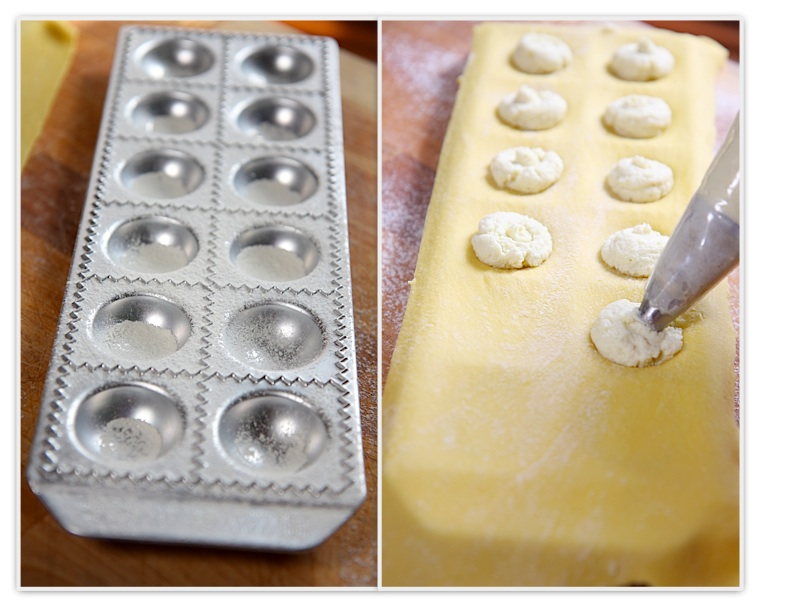
\includegraphics[scale=0.5]{images/raviolimoldwithfilling.jpg}
			\caption{Ravioliplatta för manuell fyllning av Ravioli}
			\label{ravioliplatta}	
		\end{center}
	\end{figure}
En annan typ av maskin som illustreras på figur~\ref{pastamaskin}, är väldigt stor och priset är högt som medför att de inte kan användas av hushåll.

Idén bakom detta projekt baseras på behovet av en Raviolimaskin hemma. Tanken är att utveckla en liten och relativ billig Raviolimaskin som kan vara användbar hemma.
 		\begin{figure}[h]
 			\begin{center}
 				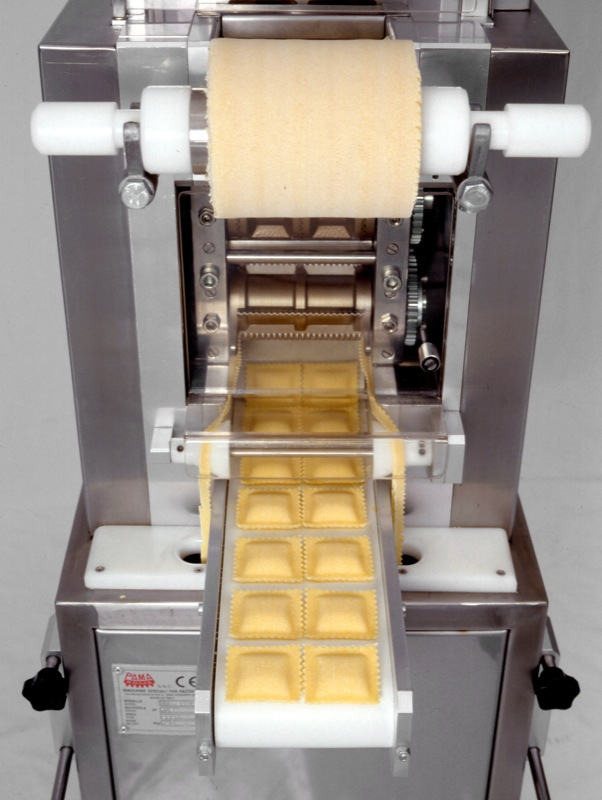
\includegraphics[scale=3]{images/pastamachine.jpg}
 				\caption{Industriell Pasta-/Raviolimaskin}
 				\label{pastamaskin}	
 			\end{center}
 		\end{figure} 

\section{Syfte och mål} % Goals
\\*

Detta projekts syfte är att utveckala en Ravioli maskin som (gör det mesta som en industeriell maskin gör men det ska vara)är rätt anpassad till hushåll i storleken, priset och användbarheten. Det är tänkt att användaren kan använda olika typer av ifyllnings material på maskinen.\\*

Maskinen är tänkt att göra det mesta av processen själv, genom att fylla Ravioli degar med ifyllnings material och stänger dem i slutet.



\section{Avgränsningar} % Constraints

Eftersom tiden är låst till en deadline som inte kan flyttas , och personalresurer är begränsande 
vi kommer inte ha maskinen i metall. Vi avgränsar oss till att ha en plastmodell på slutet av projektet. För att det är rätt mycket material som måste skrivas ut på 3D-skrivare , vilket innebär att det krävs mycket tid åt varje del.

<<<<<<< HEAD
=======
En avgränsning ska vara att alla maskinens delar kommer att konstrueras med använndning av 3D-skrivare och plast som material. 
\iffalse
Eftersom existerande verktyg som används är den enda stora begränsningen den tid det tar att genomföra 
projektet. Tiden är låst till en deadline som inte kan flyttas, och personalresurser är begränsade. 
Följaktligen är kvaliteten den enda variabel som kan ändras om projektet löper risk att inte bli klar 
på utsatt tid.
\fi
>>>>>>> d29afcd0fbd569f0d8a96f491e801229ac5807ba


%-----------------------------------------------------------

\chapter{Backgrund}
\section{Existerande Raviolimaskiner}
De Raviolimaskiner som finns på marknad innehåller två huvuddelar, en pump för fyllning och en motor-driven degform. 

Ett exempel på en Raviolimaskin visas på Figuren~\ref{raviolihemma}. Den består av två cylindriska degformar och en lucka där man fyller maskinen med fyllningsmaterial. Maskinens degfomar fungerar även som pump genom att de drar in fyllningsmaterialet när man snurrar dem m.h.a. ett handtag eller en motor.
 	\begin{figure}[h]
 		\begin{center}
 			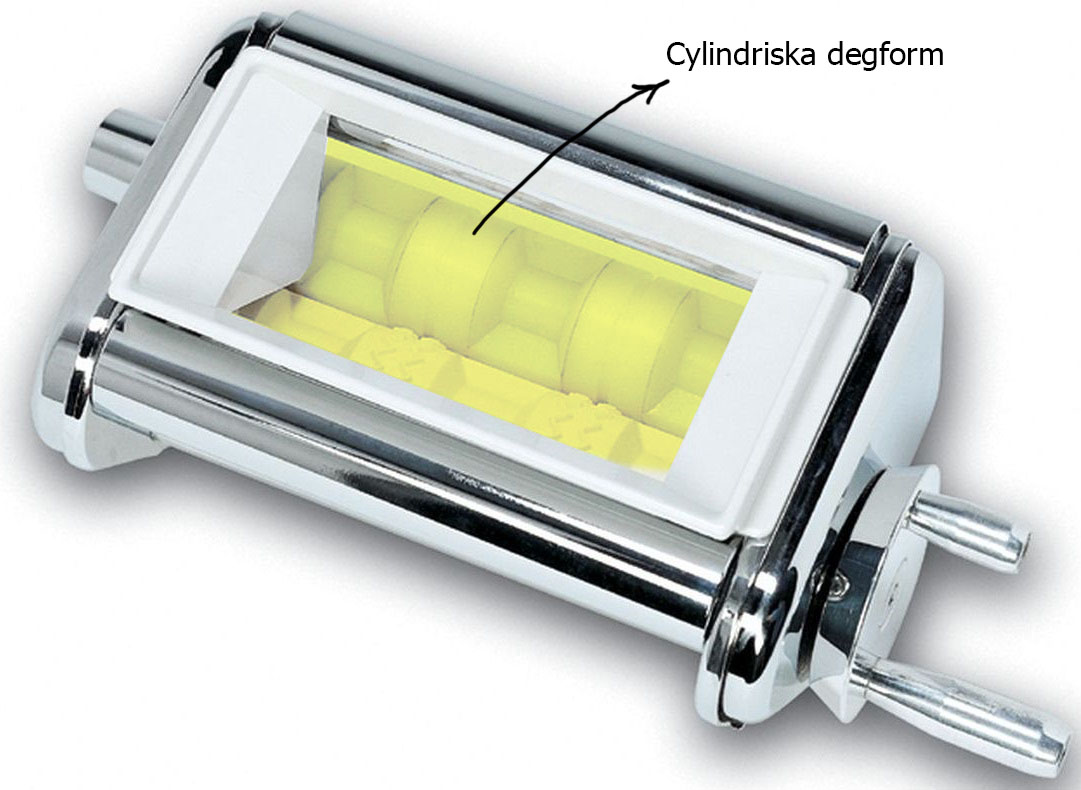
\includegraphics[scale=0.4]{images/ravioli_machine_comment.jpg}
 			\caption{Raviolimaskin bestående av två cylindriska degformar }
 			\label{raviolihemma}	
 		\end{center}
 	\end{figure}
 
Ett annat exempel på en industriell Raviolimaskin visas på figur ~\ref{industraviol_2}. Denna maskin består av en pump, två cylindriska degformar och en rullbana. Maskinen fungerar med samma princip som maskinen på det första exemplet gör och den fyller Raviolin oavbrutet under tiden som  Raviolidegen eller fyllningsmaterialet i pumpen inte har tagit slut.   .
 \begin{figure}[ht]
 	\begin{center}
 		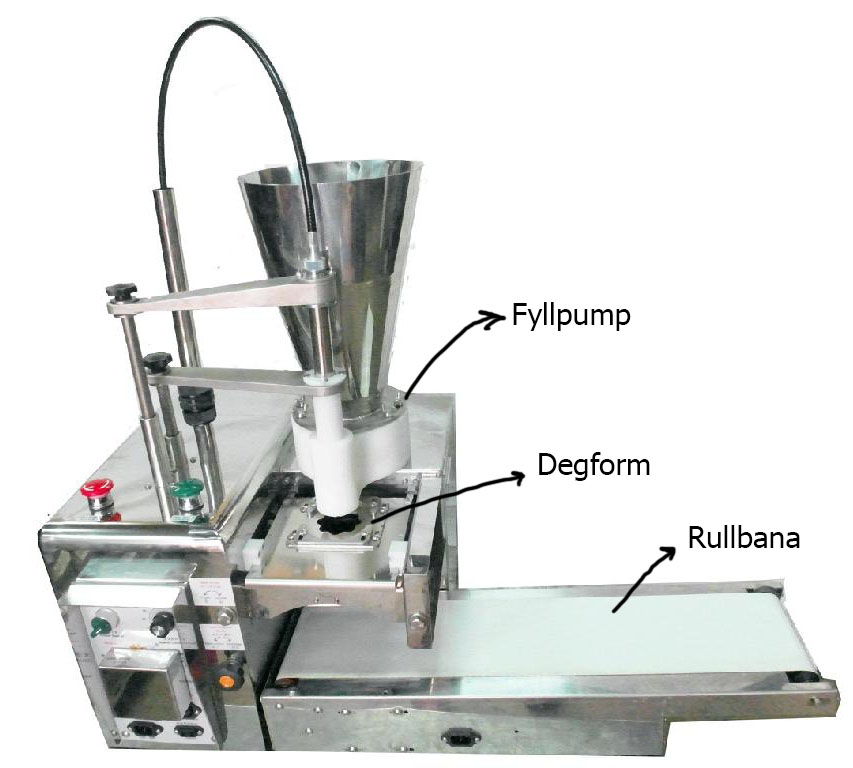
\includegraphics[scale=0.4]{images/industriell_machine_comment.jpg}
 		\caption{Industriell Raviolimaskin som gör en Ravioli i tag(ref)}
 		\label{industraviol_2}	
 	\end{center}
 \end{figure}
 
 

 
\section{Teori}
Gruppmedlemmar har undersökt olika typer av pumpar för fyllning och olika sätt som degformen kan drivas med motor. Det finns olika modeller av pumpar och två av dem är Kolvdriven och kugghjul pump. För att driva degformen med motor analyserades två typer av motorer, likströmsmotor och stegmotor. De två typer av motorer lämpar detta projekt p.g.a. de är lätt att styra och tidigare erfarenhet att använda dem i ett projekt.

En undersökning gjordes på hur man kan detektera när degformen har pressat nog Raviolidegen för att tillsluta det med tillämpning av likströmsmotor eller stegmotor.

\subsection{Olika typer av pumpar}
\textbf{Kolvpump}\\
En kolvpump pumpar ingredienserna med hjälp av en kolv som rör sig fram och tillbaka i en cylinder. Pumpen är utformad för att hantera vätskor, halvfasta och trögflytande produkter och den häller ingredienserna på degen med hjälp av ett munstycke. Doseringsvolymen på matrialet kan bestämmas genom att helt enkelt öka eller minska kolvens rörelse. Figuren~\ref{kolvpump} visar example på en kolvpump.

Födelar med pumptekniken:
\begin{itemize}
	\item Påfyllningsvolymen är exakt doserad för att minska slöseriet.
	\item Fördelningen av olika produkter och halvfasta ämnen i samma behållare är korrekt repeterbar.
	\item Pumptekniken mäter ingredienserna med precision, tack vare servodrivenkolv.
	\item Pumpen kan rengöras på plats utan nedmontering.
\end{itemize}

\begin{figure}[h]
	\begin{center}
		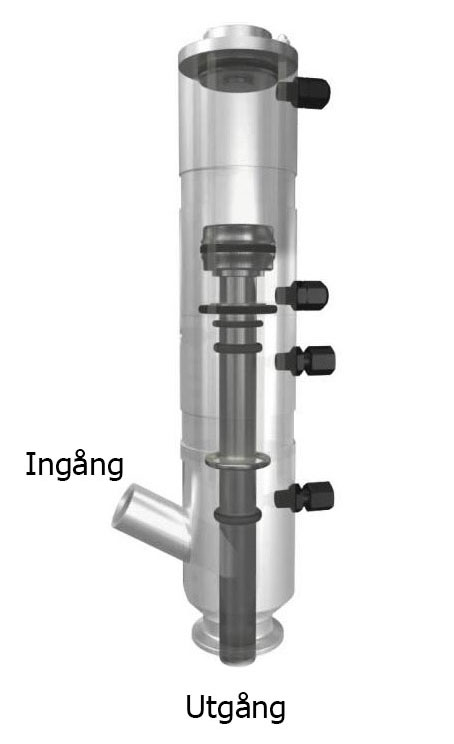
\includegraphics[scale=0.5]{images/maxresdefault.jpg}
		\caption{Kolvpump med exakt dosering för fyllningsmaterial~\cite{Dosering pump}}
		\label{kolvpump}	
	\end{center}
\end{figure}

\newpage
\textbf{Kugghjulspump}\\*
Figuren~\ref{kugghjulpump} visar en kugghjulspump som består av två kugghjul, ett drivande och ett drivet kugghjul.  Materialet följer luckorna mellan kuggarna genom pumpen. Kugghjulspumpar lämpar sig bäst för höga pumphöjder(vertikala sträcka mellan slutväxel och pump)\cite{kugghjul pump}.

Pumpen används allmänt i moderna hydrauliska system på grund av höga prestanda och lång livslängd.

\begin{figure}[h]
	\begin{center}
		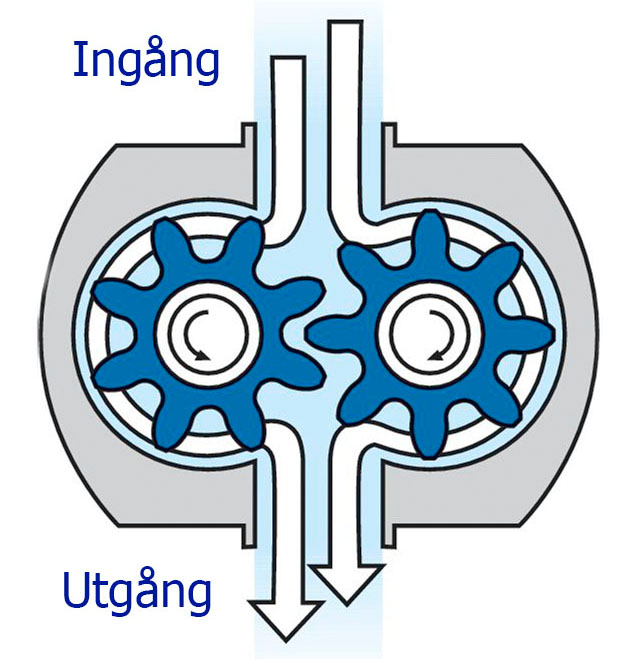
\includegraphics[scale=0.25]{images/68637(1).jpg}
		\caption{Kugghjulspump, ett av hjulen drivs av den andra}
		\label{kugghjulpump}	
	\end{center}
\end{figure} 
\subsection{Motordriven degform}
Figuren ~\ref{degform} Visar en degform för manuell fyllning av en Ravioli. Den fungerar genom att man lägger en Raviolideg på formen, efter detta läggs fyllningsmaterial på degen och sist tillsluter man degen genom att pressa formens handtag mot varandra. Degformen kan tillämpas att sluta degen automatiskt med hjälp av motorer. Lämpliga typer av motorer  är likströms- eller stegmotor.
\begin{figure}[h]
	\begin{center}
		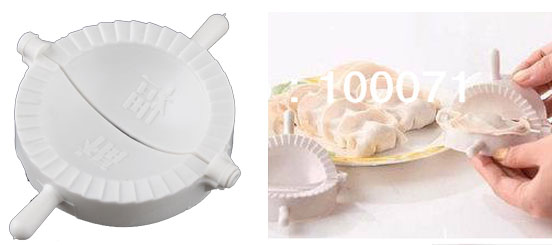
\includegraphics[scale=0.75]{images/ravioli_mould_trimed_1.jpg}
		\caption{Degform för manuell fyllning av en Ravioli}
		\label{degform}
	\end{center}
\end{figure}
\textbf{Likströmsmotor}\\*
Likströmsmotorer är den vanligaste motor som sitter i många olika produkter som leksaker, dataspel mm\cite{likstromsmotor}. Strömmen som en likströmsmotor förbrukar beror på belastningen. Denna egenskap kan användas som en sensor för att identifiera t.ex. hinder och i detta fall när degformen har pressat Raviolidegen nog för att tillsluta den.\\

\textbf{Stegmotor}\\*
Den här typen av motor liknar likströmsmotor men den skiljer sig från likströmsmotor genom en unik egenskap: stegmotor roterar ett steg vid en strömpuls. Steget minskar med ökat antal poler i statorn. Genom att beräkna antal pulsar som skickas till steg-motorn, kan man exakt positionera ett objekt \cite{stegmotor}.

\subsection{Styrenhet}
\input{chapters/mätkort}
\subsection{Kommunikation med användare}
Det finns inget specillet interface för både industriell och manuel Raviolimaskin. De flesta av maskiner använder sig av några knappar som start/stopp knapp. Här beskrivs två alternativa lösningar som man kan använda för kommunikation mellan Raviolimaskinen och användaren.\\

\textbf{Kommunikation via dator}\\
Kommunikation sker mellan en dator och maskinens styrenhet via USB. Styrenheten skickar information om maskinens status till datorn seriellt\cite{Arduinocookbook}. Datorn tar emot de inkomna seriella signaler, tolkar dem och visar information på skärmen på ett läsbart sätt för en användare.\\


\textbf{Display}\\
LCD används i olika typer av enheter. Fördelar med att använda LCD som interface är effektivitet, storlek och låg kostnad.  LCD kan kopplas direkt till plattformen, vilket är bra för maskinen som inte är stor i storleken.



\chapter{Metod}
Raviolimaskin som ska tas fram är tänkt att fylla en Ravioli i tag. Detta görs genom att utforma maskinens degform så att endast en Raviolideg kan placeras på formen. Man ska placera en Raviolideg på maskinens degform. Efter detta ska degformen hissa upp till maskinens pump. Detta görs för att minska avståndet mellan degform och maskinens pump som i sin tur minskar materialslöseriet. I näst ska fyllningsmaterialet pumpas på Raviolidegen som är placerad på formen. Till slut hissas ner degformen och sluter till degformen. Figuren~\ref{blockschema} maskinens olika tillstånd.

\begin{figure}[ht]
	\begin{center}
		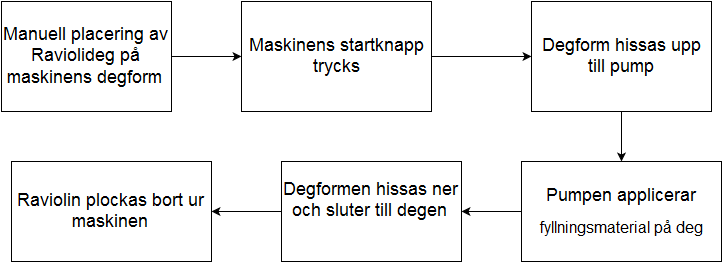
\includegraphics[scale=0.8]{images/blockschema.png}
		\caption{Maskinens olika tillstånd}
		\label{blockschema}	
	\end{center}
\end{figure}

\section{Maskinens pump för fyllning}
Val av pump görs med tanke på Raviolimaskinens behov och tillverknings möjligheten. Kolvpump kan pumpa fyllningsmaterialet med högre noggrannhet än kugghjulspumpar. Däremot behöver man endast en motor för att driva kugghjuls pump i jämförelse med två motorer som ska behövas för en kolvpump.

För detta projekt ska en variant av kugghjuls pump tillverkas som består av endast ett kugghjul. Pumpen ska tillämpas för Raviolimaskinen genom att implementera ett filter i pumpen som ska filtrera eventuell vätska i fyllningsmaterialet. Kugghjuls pump ska drivas med användning av en stegmotor som kan positionera pumpens kugghjul exakt i den önskade positionen.

\section{Motordriven degform}
Maskinens degform ska stänga Raviolidegen med hjälp av två likströmsmotorer. Motorers rotationsenergi ska överföras till degformen med användning av kugghjulsväxel.  Genom avläsning av motorers ström kan man upptäcka när formen har pressat Raviolidegen tillräcklig mycket.\\

Det är också tänkt att implementera möjligheten att hissa upp och ner maskinens degform. Detta görs för att minska avstånd mellan maskinens degform och pump. För att genomföra detta ska en kuggväxel bestående av två kugghjul och två kuggsträngar användas, se figur.~\ref{motordrivendegform}

\begin{figure}[ht]
	\begin{center}
		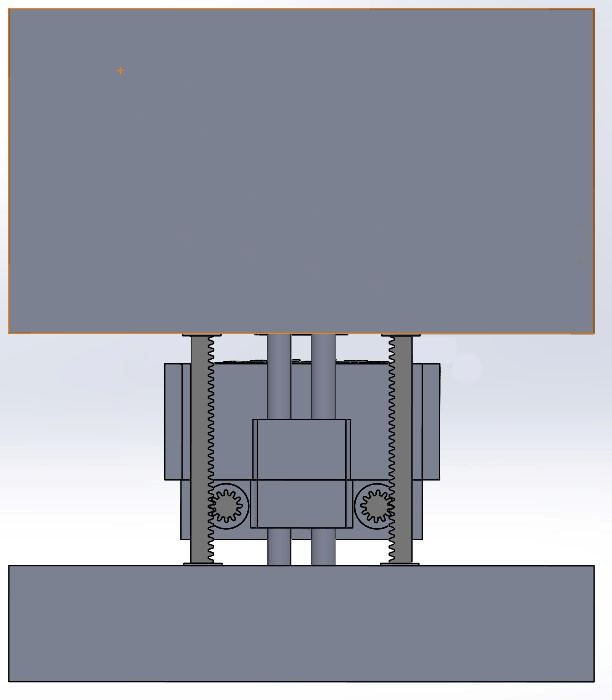
\includegraphics[scale=0.8]{images/maskinenshiss.jpg}
		\caption{Industriell Raviolimaskin som gör en Ravioli i tag(ref)}
		\label{motordrivendegform}	
	\end{center}
\end{figure}

\section{Design av maskin}
Maskinens alla delar ritas med användning av ”SolidWorks” som är ett CAD program. Utöver möjligheten att rita möjliggör SolidWorks simulering av de ritade delarna. Med denna egenskap kan man kontrollera och se hur maskinenes olika delar fungerar ihop som en maskin. På programmets simulator kan man påverka en visuell kraft på en del och avsyna hur den reagerar innan man konstruerar en del.
\begin{figure}[ht]
	\begin{center}
		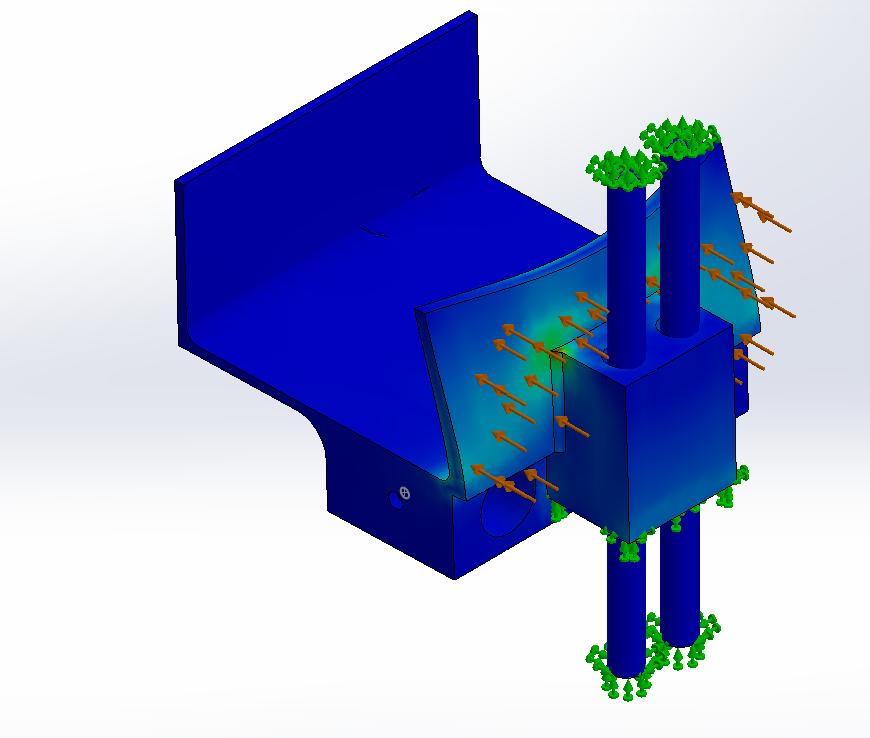
\includegraphics[scale=0.8]{images/hissEdited.png}
		\caption{Exempel på visuell kraf påverkat på en del i SolidWorks}
		\label{simulering}	
	\end{center}
\end{figure}
\section{Tillverknings av maskinens delar}
Maskinens delar är tänkt att printas genom att använda en 3D-skrivare. Fördelen med 3D-printern är att det är enkelt att printa en del som är svårt att tillverka med hand med minst fel. Det blir betydligt snabbare att printa med 3D-skrivare i jämförelse med tillverkning av samma del med hand i en verkstad. 
\section{Sensor}
I detta projekt används tre olika metoder för att identifiera motorers position och för säkerhet av maskinen.
\subsection{Strömavläsning}
Strömmen som går genom en likströmsmotor ökar med ökad belastning. Ett exempel är motorer som ska hissa upp och ner maskinens degform, se figur~\ref{maskinens_baksida_metod}. När de har hissat upp degformen till ändläge på kuggsträngar, ökar strömmen i motorer som kan avläsas för att identifiera motorers position.
\subsection{IR-sensor}
Det ska tas fram en IR-sensor genom att använda en IR-sändare som skickar ut IR-signaler och en fototransistor som tar emot IR signaler. Under tiden som fototransistor tar emot signaler definieras som normalläge. Så fort som fototransistor inte tar IR-signaler är då ett objekt mellan sensorer.


\section{Styrenhet}
Enligt kravspecifikation jämfördes de tre olika alternativen för att välja på vilken processor lämpar sig bäst för detta projekt med tanke på mögligheten för sekvensstyrning.

PLC är ett system för automationteknik, som används mest för styrning och reglering för industriella processor. Däremot används mikrokontroller Arduiono och Raspberry pi för inbyggda system. Det som är bra med Arduino och Raspberry pi jämfört med PLC är att kostnadpriset för de är inte så mycket, vilket är det viktig för detta ska vara en hemanvändare maskin.

Gemensama fördelar mellan Arduino och Raspberry pi
\begin{itemize}
	\item Gott om anslutningsmögligheter(både analogt och digitalt).
	\item Den är relativt billig samt är enkel att programmera.
	\item Bra för styrning av många motorer genom PWM.
	\item Möglighet för sekvensstyrning.
\end{itemize}

 Arduino kräver inte specillet operativsystem medans Raspberry pi operativsytem är baserad på Linux. Fördelen med  Arduino är att det har inbyggt minne men Rasberry pi använder sig av ett extern SD kort. Arduino har realtid och analog funktioner som Rassbery inte har. Pi är inte så flexibel, t.ex.för att läsa analoga sensorer kräver extra hårdvara stöd.


%\section{Blockschema}
%\section{Testning}

\chapter{Hittlis resultat}
\section{Maskinens design}
Ritning av maskinens delar är 90 \% klara. Det återstår småändringar som förekomma under tillverknings av delarna. Figuren ~\ref{helmaskin} visar en översikt av maskinens ritning på SolidWorks.

\begin{figure}[h]
	\begin{center}
		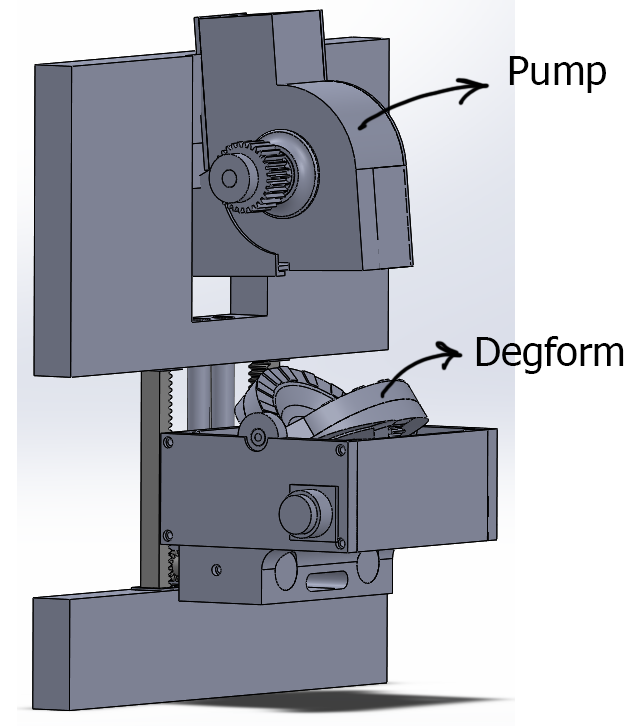
\includegraphics[scale=0.75]{images/hela_maskin.png}
		\caption{Översikt av hela maskin bestående av pump, degform och hiss}
		\label{helmaskin}
	\end{center}
\end{figure}


\begin{figure}[h]
	\begin{center}
		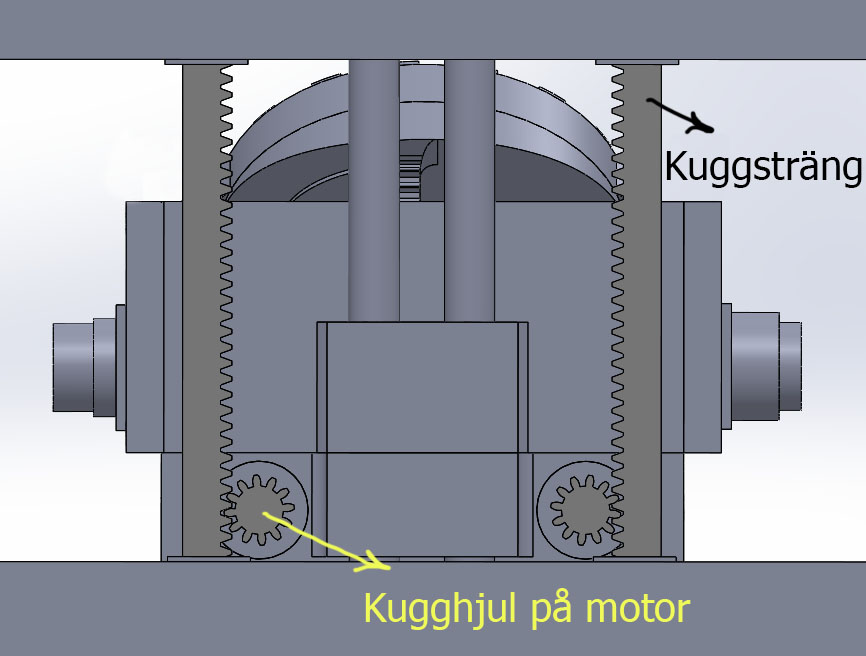
\includegraphics[scale=0.75]{images/maskinBaksida.jpg}
		\caption{Översikt av hela maskin bestående av pump, degform och hiss}
		\label{helmaskinbaksida}
	\end{center}
\end{figure}

%\chapter{Tidsplan}
%Examenarbetet krävs 20 timmar arbetsinsats i veckan. Därför måste läggas minst 350 timmar 
för att kunna klara arbetet. Följande är en grovplanering till projektet med tanke på de olika uppgifter som ska göras. \\


\begin{figure}[h]
	\begin{center}
		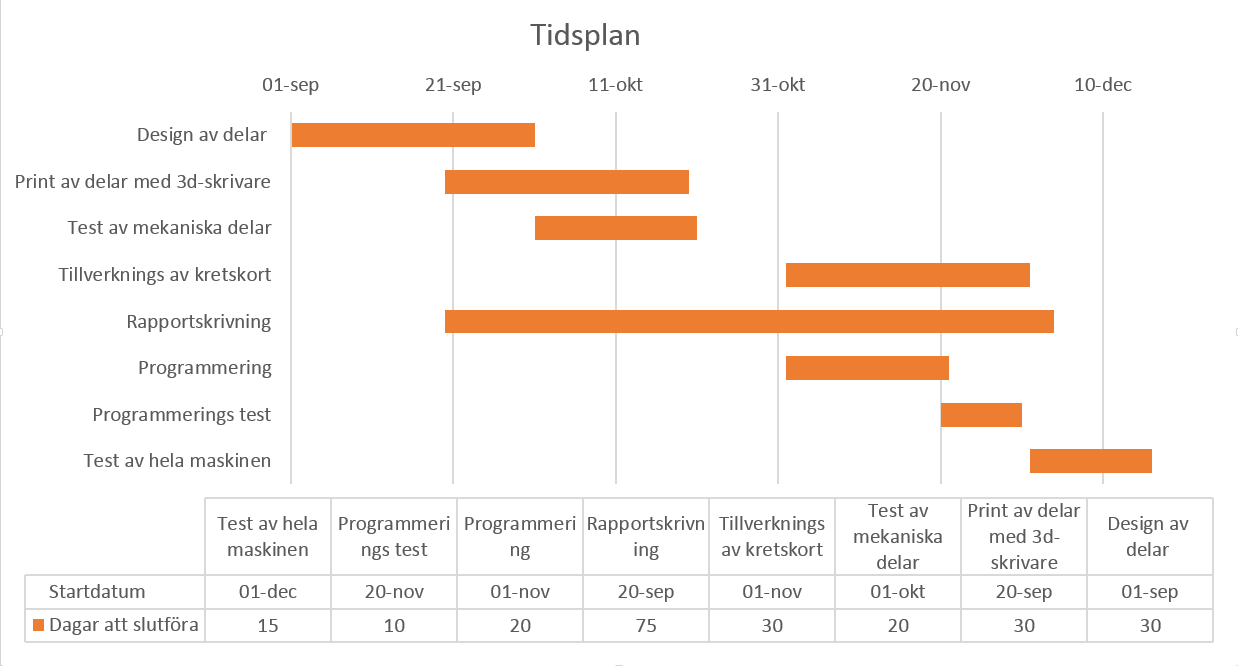
\includegraphics[scale=0.5] {images/tidsplan.png}
		\label{Tidsplan}	
	\end{center}
\end{figure}
\section{kommunikation och styrning}
Prototypen består av motorer, kugghjular, sensorer och mikrokontroller. Centralt i det systemet bestämdes att använda Arduino due som ska kommunicera med alla elektriska komponenter.

Anledningen för valet av Arduino due är att den fyller specifikationkraven som ställdes för styrenheten. Utöver dessa finns tillräcklig antal portar för att koppla motorer och sensorer samt att det kan bestämmas farten på hissen som går upp och ner genom PWM signalen. Arduino är en liten plattform, vilken är bra för maskinens begränssad storlek. Tidigare erfanhet att använda och programmera med Arduino samt mögligheten att programmera i C/C++ var också en fördel.

För att kunna kommunicera med användaren används en display som heter 3.2" TFT LCD Touch shield, vilket hjälper användaren att övervaka maskinens tillstånd och eventuella fel.

Figuren~\ref{flodesschma} visar systemets flödesschema.

\begin{figure}[ht]
	\begin{center}
		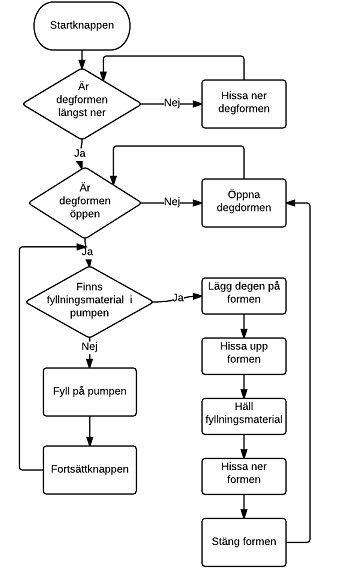
\includegraphics[scale=1.7]{images/Flowchart.png}
		\caption{Systemets flödesschema.}
		\label{flodesschma}	
	\end{center}
\end{figure}
%\section{Design}


%\begin{itemize}
% \item Krav nr 1: Bygga en reglercentral som ska ersätta innedelen.
 %\item Krav nr 2: Reglercentralen ska kommunicera med utedelen enbart med RS-485 via kontakter F1 och F2.
% \item Krav nr 3: Reglercentralen ska hantera två insignaler. En analog signal mellan 0 till 10 volt och en digital signal.
% \item Krav nr 4: Reglercentralen ska översätta kompressorns frekvens så att tex 1 volt analog insignal motsvarar 10\% av kompressorn kapacitet, 2 volt 20 \% osv.
% \item Krav nr 5: Värme eller kylläge på utedelen ska väljas med den digitala insignalen till centralen.\\*
%\end{itemize}

\backmatter
% Referenser--------------------------------------------------------------------
 \bibliographystyle{99}
\begin{thebibliography}{1}
\bibitem{engproc}
\href{http://www.wisegeek.com/what-is-ravioli.htm}{http://www.wisegeek.com/what-is-ravioli.htm}, Engproc

\bibitem{ravioliplatta}
\href{http://www.clasohlson.com/se/Ravioliform/44-1053?userSelection=B2C\&rememberCookie=false}{http://www.clasohlson.com/se/Ravioliform/44-1053?userSelection=B2C\&rememberCookie=false}, Ravioliplatta

\bibitem{induRavioliMaskin}
\href{http://www.pamaroma.com/raviolipastamachine.htm}{
	http://www.pamaroma.com/raviolipastamachine.htm},Ravioli restaurang maskin	
\bibitem{raviolimaskinbutik}
\href{http://www.kitchenaid.com/shop/-[KRAV]-400107/KRAV/}{http://www.kitchenaid.com/shop/-[KRAV]-400107/KRAV}, kitchenAid

\bibitem{diytrade}
\href{http://www.diytrade.com/china/pd/8029124/Desktop_dumpling_machine.html}{http://www.diytrade.com/china/pd/8029124/Desktop_dumpling_machine.html},Industriell Raviolimaskin

\bibitem{Dosering pump}
\href{http://gb.pcm.eu/en/food-applications/filling-dosys-technology.html}{http://gb.pcm.eu/en/food-applications/filling-dosys-technology.html},Dosering pump

\bibitem{kugghjul pump}
\href{http://hj.diva-portal.org/smash/get/diva2:219806/FULLTEXT01.pdf}{http://hj.diva-portal.org/smash/get/diva2:219806/FULLTEXT01.pdf},kugghjul pump


\bibitem{likstromsmotor}
\href{http://www.drivteknik.nu/skolan/motor/stegmotor}{http://www.drivteknik.nu/skolan/motor/stegmotor}, Likströmsmotor
\bibitem{stegmotor}
\href{http://www.ne.se.ezproxy.bib.hh.se/uppslagsverk/encyklopedi/l\%C3\%A5ng/stegmotor}{http://www.ne.se.ezproxy.bib.hh.se/uppslagsverk/encyklopedi/l\%C3\%A5ng/stegmotor}, Stegmotor

\bibitem{Maskinstyrning}
\href{http://www.iei.liu.se/indprod/grundutbildning/tmmi32/plc_programering_och_opto22_material/1.212886/Sekvensstyrning.pdf }{http://www.iei.liu.se/indprod/grundutbildning/tmmi32/plc_programering_och_opto22_material/1.212886/Sekvensstyrning.pdf }, Maskinstyrning



%\href{http://www.lawicel-shop.se/dept/Arduino_74952/SWE/SEK}{http://www.lawicel-shop.se/dept/Arduino_74952/SWE/SEK},Arduino
\bibitem{Arduino1}
\href{https://learn.sparkfun.com/tutorials/what-is-an-arduino}{https://learn.sparkfun.com/tutorials/what-is-an-arduino },Arduino1

\bibitem{Arduino2}
\href{http://www.lawicel-shop.se/dept/Arduino_74952/SWE/SEK}{http://www.lawicel-shop.se/dept/Arduino_74952/SWE/SEK},Arduino2

\bibitem{Raspberry1}
\href{http://computers.tutsplus.com/tutorials/controlling-dc-motors-using-python-with-a-raspberry-pi--cms-20051}{http://computers.tutsplus.com/tutorials/controlling-dc-motors-using-python-with-a-raspberry-pi--cms-20051}, Raspberry1

\bibitem{Programmable Logical Controller}
\href{http://publications.lib.chalmers.se/records/fulltext/159868.pdf}{http://publications.lib.chalmers.se/records/fulltext/159868.pdf}, plc

\bibitem{Arduinocookbook}
\href{http://onlinevideolecture.com/ebooks/index.php?subject=Arduino  }{http://onlinevideolecture.com/ebooks/index.php?subject=Arduino},Arduinocookbook,Michael Margolis, sidan 80

\bibitem{Arduino3}
\href{https://learn.sparkfun.com/tutorials/what-is-an-arduino}{https://learn.sparkfun.com/tutorials/what-is-an-arduino},Arduino3
\bibitem{Raspberry}
\href{https://www.raspberrypi.org/help/what-is-a-raspberry-pi/}{https://www.raspberrypi.org/help/what-is-a-raspberry-pi/},Raspberry






\end{thebibliography}


\end{document}
